\chapter{Submission 2 ($21^{st}$ March)}
\section{Progress so far}
\label{sec-prog-so-far}
\begin{itemize}
 \item We have throughly read the paper mentioned in \ref{sec-feasibility}, and implemented the algorithm.
 \item There were some problems in dividing the dataset as the ISEAR dataset mentioned in \ref{sec-dataset}.
 \begin{itemize}
  \item Has a total of 7 emotion classes, but for the sake of simplicity we chose to model only 3 of them.
  \item Out of the 7 classes, 6 are negative emotions (\textbf{sadness, guilt, shame, fear, anger, disgust}) and only 1 positive (\textbf{joy}).
  \item We had 2 choices now, either to divide the leftover data for 4 classes into the 2 negative ones, we've chosen (\textbf{anger,sadness}).
  \item Doing this caused a lot of misclassification, so after some research, we've currently left out 2 emotions - \textbf{guilty,fear}.
 \end{itemize}
 \item We wrote Python code to correctly implement the vector space model algorithm mentioned in \ref{subsec-high-level-alg}. We are working collaboratively and have set up a github repo to house all the data, report and code. The link is \url{https://github.com/sm88/mlproject}.
 \item Due to the above mentioned reason for less data, we are looking into some more datasets, mentioned in the paper namely, the Wordnet-Affect dataset and the Semeval dataset.
 \item The wordnet database is not available easily as we need to fill out a form, which after review will enable us to download.
 \item We have throughly cleaned the dataset, which initially had many problems. A few major ones that we solved are:
 \begin{itemize}
  \item Many sentences were of form ``No Response'', which provides no information whatsoever.
  \item There were some scattered braces and square brackets as well as some non-ascii characters, that took a while to catch.
  \item Some sentences were repeated for multiple classes.
 \end{itemize}
 \item We have done some preliminary tests on the training data itself and the results seem promising (see table \ref{tab-confusion}).
\end{itemize}
\begin{center}
	\begin{figure}[ht!]
	\label{fig-clean-dataset}	
	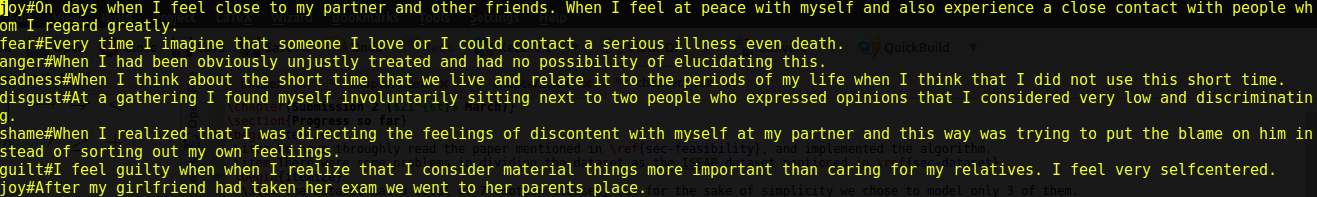
\includegraphics[width=18cm,scale=0.5]{data.png}
	\caption{Cleaned partial ISEAR dataset}
	\end{figure}
\end{center}	
\vspace*{-1cm}
\begin{table}[ht!]
  \centering
  \label{tab-confusion}
  \begin{tabular}{c|c|c|c}
  & \textbf{anger} & \textbf{sadness} & \textbf{joy}\\
  \hline
  \textbf{anger} & 1432 & 413 & 318 \\
  \textbf{sadness} & 384 & 2221 & 620 \\
  \textbf{joy} & 28 & 61 & 1001 \\
  \end{tabular}
  \caption{Confusion matrix for training set}
\end{table}
\vspace*{-0.5cm}
\begin{table}[ht!]
  \centering
  \label{tab-accuracy}
  \begin{tabular}{c|c}
  \textbf{Emotion} & \textbf{Accuracy \%} \\
  \hline
  anger & 66 \\
  sadness & 69 \\
  joy & 92
  \end{tabular}
  \caption{Per emotion class accuracy for training set}
\end{table}
\subsection{Implementation Details}
\begin{itemize}
 \item We are building the solution in python v3.4.2, using \textbf{nltk, sklearn}
 \item Currently we have a shell script to clean the data. Some cleaning has been done manually.
 \item We have well structured code with clear flow control through judicious use of functions. Data and code placed in separate folders.
 \item We will be converting the code to classes so as to make it easy to switch classifiers(which we'll build later) with ease.
\end{itemize}
\subsection{Other Info}
\begin{itemize}
 \item We believe that with bigger dataset, we'll be able to improve the accuracy of \textbf{anger, sadness} further.
 \item The training time is around a minute and query time is about a second, depending on the length of the sentence.
 \item Our document vectors mentioned in \ref{subsec-high-level-alg} are sparse in nature (total number of words compared to words in a sentence) as a result of which we have excellent opportunities to optimize our implementation.
\end{itemize}
\section{Plan for the rest of the semester}
\label{sec-plan-for-sem}
\begin{enumerate}
 \item We will try and find more patterns in the dataset like the one shown in the paper. There they've created new words from negative verbs. For example, the input sentence ``I don't love you.'' is transformed to ``I do not love you.'' which is again transformed to ``I do NOTlove you''. Here we see that finally a new word \emph{NOTlove} has been created. Authors claim this helps increase accuracy.
 \item We will find set differences between various classes on basis of words (words unique to each emotion class), and remove them from stop words list for accurate predictions.
 \item Make the training process more efficient by using sparse arrays instead of arrays with all the terms in the lexicon.
 \item We will implement naive baye's classifier and try bi-gram, tri-gram etc approaches.
 \item We will also try and see if we can get some better results with decision trees method, as some words uniquely determine the emotion of a sentence.
 \item We will try to get our hands on some additional datasets, mentioned in \ref{sec-prog-so-far} so as to get more data for testing and also supplement our training data.
 \item Since this is a high dimensional feature space, SVM can be hoped to yield good results. If time permits, we will use it.
 \item If time permits, we will develop some application to showcase our models, which will allow changing models dynamically.
 \item We will also do sentiment analysis of our dataset where we will just check the accuracy of negative and positive emotions(binary classification).
\end{enumerate}
\section{Pointers to literature}
\begin{itemize}
 \item The main dataset and paper are mentioned in section \ref{sec-feasibility} and \ref{sec-dataset} respectively.
 \item The wordnet-affect dataset can be accessed from \url{http://wndomains.fbk.eu/wnaffect.html} although we need to fill out some forms before we are granted a download link.
 \item The Semeval task 14, is a medical dataset available at \url{http://alt.qcri.org/semeval2015/task14/index.php?id=data-and-tools}.
 \item Multinomial naive baye's using \textbf{tf-idf} technique can be found at \url{http://sebastianraschka.com/Articles/2014_naive_bayes_1.html}.
 \item As mentioned in section \ref{sec-plan-for-sem}, SVM could be useful for classification. The paper at \url{http://www.cs.cornell.edu/people/tj/publications/joachims_98a.pdf} presents a good use case.
 \item For naive baye's we could also add the chi-squared test for confidence computation. Some details are outlined in \url{http://www.dis.uniroma1.it/~leon/didattica/webir/IR11.pdf}.
 \item Code listing is attached and is publicly available at \url{https://github.com/sm88/mlproject}.
\end{itemize}



